\begin{IEEEbiography}[{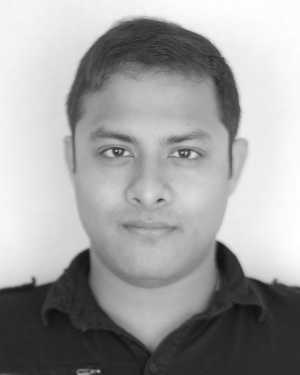
\includegraphics[width=1in,height=1.5in,clip,keepaspectratio]{./images/sange.png}}]{Sangekar Mehul Naresh}
(M’10) received the M.Sc. degree in underwater robotics and Ph.D. degree in ocean technology from The University of Tokyo, Japan, in 2010 and 2014, respectively. He is  working at present as a project researcher at the Thornton Lab, Institute of Industrial Science, The University of Tokyo. Currently, he works on techniques for intelligent, multi-layer resolution mapping of the seafloor using autonomous underwater vehicles. He is also working on developing algorithms for analysis of high resolution seafloor bathymetry and correlating it with other measured seafloor parameters.  
\end{IEEEbiography}

\vskip 0pt plus -1fil

\begin{IEEEbiography}[{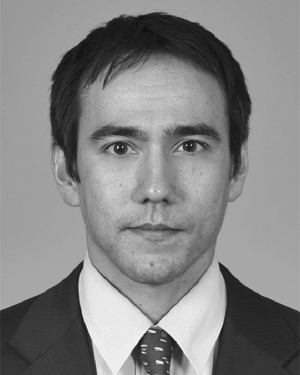
\includegraphics[width=1in,height=1.5in,clip,keepaspectratio]{./images/thorn.png}}]{Thornton Blair}
(M’07) received the B.Eng. degree in ship science and the Ph.D. degree in underwater robotics from The University of Southampton, Southampton, U.K., in 2002 and 2006, respectively. He is at present an Associate Professor at the the University of Southampton and also affiliated with the  Ocean Perception Laboratory, Institute of Industrial Science, The University of Tokyo. His research interests involve the development of in-situ sensors and data processing techniques for integrated acoustic, visual, and chemical survey of marine minerals and environment monitoring. He is dedicated to fielding real systems in real environments and overcoming bottlenecks in the flow of information from data collection to human interpretation.
\end{IEEEbiography}

\vskip 0pt plus -1fil

\begin{IEEEbiography}[{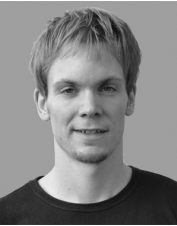
\includegraphics[width=1in,height=1.5in,clip,keepaspectratio]{./images/boden.png}}]{Adrian Bodenmann}
(M’09) received the M.Sc. degree in microengineering from the Ecole Poly- technique Fédérale de Lausanne (EPFL), Lausanne, Switzerland, in 2009. He is a Project Researcher at the Underwater Technology Research Center, University of Tokyo, Tokyo, Japan. Currently, he works on 3-D seafloor visual mapping and automated data processing algorithms, and is developing a long-range 3-D color mapping system for wide area marine surveys.
\end{IEEEbiography}

\vskip 0pt plus -1fil

\begin{IEEEbiography}[{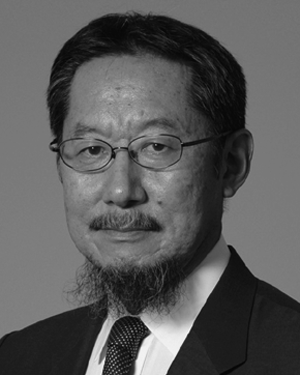
\includegraphics[width=1in,height=1.5in,clip,keepaspectratio]{./images/ura.png}}]{Ura Tamaki}
(M’91–SM’02–F’07) graduated from the Faculty of Engineering, The University of Tokyo, Japan, in 1972 and received the degree of Doctor of Engineering from the same university in 1977. He is at present the Professor emeritus of The University of Tokyo and  Director, Distinguished Professor of Center for Socio-Robotic Synthesis, Kyushu Institute of Technology, and Director of Underwater Technology Center of National Maritime Research Institute. He has developed various types of Autonomous Underwater Vehicles (AUVs) and related application technologies including navigation methods, a new sensing method using a chemical sensor, precise seafloor mapping methods, a precise seabed positioning system with a resolution of a few centimeters, a new sensing system of the thickness of cobalt-rich crust, etc. Finally, he exemplified using these technologies that AUVs are practicable and valuable tools for deep-sea exploration.
\end{IEEEbiography}